%%%%%%%%%%%%%%
% Reproducible research workflow + link commands
% Christopher Gandrud
% Updated 19 November 2012
%%%%%%%%%%%%%%

% Define colors for figure
%% Color palette (GnBU) chosen using ColorBrewer 2.0
%% See: http://colorbrewer2.org/
%% Not used in the print version
\definecolor{Blue}{HTML}{7BCCC4}
\definecolor{LiteBlue}{HTML}{A8DDB5}
\definecolor{DarkBlue}{HTML}{08589E}

\definecolor{GrayLine}{HTML}{BDBDBD}

% Set node styles
%% Workflow stage nodes
\tikzstyle{Stage} = [draw=Blue, 
                     %fill=Blue, 
                     rectangle, 
                     text width=7em, 
                     inner sep=0.5cm, 
                     font=\small]

% Raw Data nodes
\tikzstyle{RawData} = [draw=LiteBlue, 
                       %fill=LiteBlue, 
                       decorate,
                       decoration={random steps,
                                   segment length=2pt,
                                   amplitude=2pt},
                       inner sep=0.25cm, 
                       font=\scriptsize]
                    
% Separator line style
\tikzstyle{sepline} = [draw,
                        very thick,
                        color=GrayLine]
                        
% Link command nodes       
\tikzstyle{Links} = [draw=none, 
                          text width=6em,
                          text=DarkBlue,
                          font=\small]

% Begin tikz picture
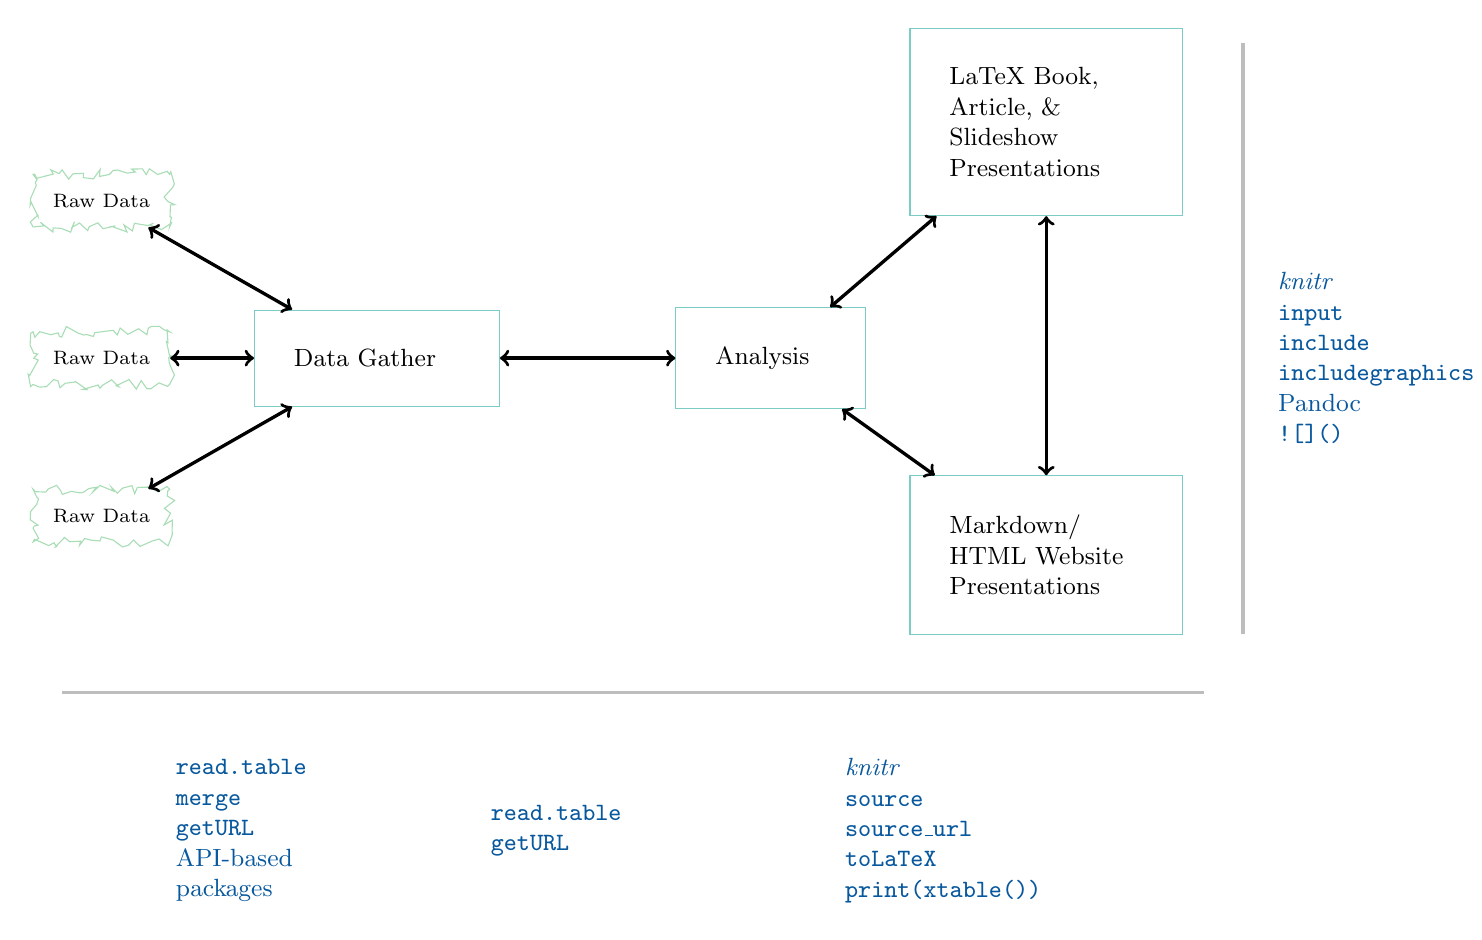
\begin{tikzpicture}

    % Raw Data Nodes
    \node (Data1) at (-3, 7) [RawData]{Raw Data};
    \node (Data2) at (-3, 5) [RawData]{Raw Data};
    \node (Data3) at (-3, 3) [RawData]{Raw Data}; 
    
    % Workflow stage nodes
    \node (DataGather) at (0.5, 5) [Stage, text width= 6em]{Data Gather};
    \node (Analysis) at (5.5, 5) [Stage, text width= 4em]{Analysis};
    \node (Presentation1) at (9, 8) [Stage]{LaTeX Book, \\ Article, \& \\ Slideshow \\ Presentations};
    \node (Presentation2) at (9, 2.5) [Stage]{Markdown/ \\ HTML Website \\ Presentations};

    % Lines
    \draw [<->, very thick] (Data1) -- (DataGather);
    \draw [<->, very thick] (Data2) -- (DataGather);
    \draw [<->, very thick] (Data3) -- (DataGather);
    \draw [<->, very thick] (DataGather) -- (Analysis);
    \draw [<->, very thick] (Analysis) -- (Presentation1);
    \draw [<->, very thick] (Analysis) -- (Presentation2);
    
    \draw [<->, very thick] (Presentation1) -- (Presentation2);
    
    \path [sepline] (-3.5, 0.75) -- (11, 0.75);
    \path [sepline] (11.5, 9) -- (11.5, 1.5);
    
    % Link command nodes
 
    \node (pres) at (13, 5) [Links]{{\emph{knitr}} \\ \texttt{input} \\ \texttt{include} \\ \texttt{includegraphics} \\ Pandoc \\ \texttt{![]()}};
    \node (knitr) at (7.5, -1) [Links]{ {\emph{knitr}} \\ \texttt{source} \\ \texttt{source\_url} \\ \texttt{toLaTeX} \\ \texttt{print(xtable())} };
    \node (readData) at (3, -1) [Links]{ \texttt{read.table} \\ \texttt{getURL} };
    
    \node (importData) at (-1, -1) [Links]{\texttt{read.table} \\ \texttt{merge}\\ \texttt{getURL} \\ API-based packages};

  
\end{tikzpicture}